


\section{Experiments}
\label{sec:Experiments}
\subsection{Experimental Setup}



\begin{table*}[!t]
\centering
\small
\setlength{\tabcolsep}{2.25pt}
\renewcommand{\arraystretch}{1.08}

% Local vertical separators. They appear only in normal/header rows,
% and disappear automatically in section-title rows with \multicolumn.
\newcommand{\metricssep}{\rule[-0.35em]{0.35pt}{1.55em}}

\resizebox{\textwidth}{!}{
\begin{tabular}{@{}l c c c c c c c c c c c c c c c c@{}}
\toprule
\multirow{2}{*}{\textbf{Models}}
& \multirow{2}{*}{\textbf{Params.}}
% \textbf{Models} & \textbf{Params.} 
& \metricssep
& \multicolumn{6}{c}{\textbf{DPG-Bench}}
& \metricssep
& \multicolumn{7}{c}{\textbf{GenEval}} \\
\cmidrule(lr){4-9} \cmidrule(lr){11-17}
&
& \metricssep
& \textbf{Global} & \textbf{Entity} & \textbf{Attribute} & \textbf{Relation} & \textbf{Other} & \textbf{Overall}
& \metricssep
& \textbf{1-Obj.} & \textbf{2-Obj.} & \textbf{Count} & \textbf{Colors} & \textbf{Position} & \textbf{Attr.} & \textbf{Overall} \\
\midrule

\multicolumn{17}{@{}>{\columncolor{gray!12}}c@{}}{\textit{Generation-only Models}} \\

PixArt-$\alpha$ \cite{chen2024pixart}
& 0.6B
& \metricssep
& 74.97 & 79.32 & 78.60 & 82.57 & 76.96 & 71.11
& \metricssep
& 0.98 & 0.50 & 0.44 & 0.80 & 0.08 & 0.07 & 0.48 \\

SDXL \cite{podell2024sdxl}
& 3.5B
& \metricssep
& 83.27 & 82.43 & 80.91 & 86.76 & 80.41 & 74.65
& \metricssep
& 0.98 & 0.74 & 0.39 & 0.85 & 0.15 & 0.23 & 0.55 \\

Hunyuan-DiT \cite{li2024hunyuan}
& 1.5B
& \metricssep
& 84.59 & 80.59 & 88.01 & 74.36 & 86.41 & 78.87
& \metricssep
& -- & -- & -- & -- & -- & -- & -- \\

% Playground v2.5 \cite{li2024playground}
% & --
% & \metricssep
% & 83.06 & 82.59 & 81.20 & 84.08 & 83.50 & 75.47
% & \metricssep
% & -- & -- & -- & -- & -- & -- & -- \\

DALL-E 3 \cite{betker2023improving}
& --
& \metricssep
& 90.97 & 89.61 & 88.39 & 90.58 & 89.83 & 83.50
& \metricssep
& 0.96 & 0.87 & 0.47 & 0.83 & 0.43 & 0.45 & 0.67 \\

SD3-Medium \cite{esser2024scaling}
& 2B
& \metricssep
& 87.90 & 91.01 & 88.83 & 80.70 & 88.68 & 84.08
& \metricssep
& 0.99 & 0.94 & 0.72 & 0.89 & 0.33 & 0.60 & 0.74 \\

Emu3-Gen \cite{wang2024emu3}
& 8B
& \metricssep
& 85.21 & 86.68 & 86.84 & 90.22 & 83.15 & 80.60
& \metricssep
& 0.98 & 0.71 & 0.34 & 0.81 & 0.17 & 0.21 & 0.54 \\

FLUX.1-dev$^\dagger$ \cite{blackforestlabs_flux}
& 12B
& \metricssep
& 74.35 & 90.00 & 88.96 & 90.87 & 88.33 & 83.84
& \metricssep
& 0.98 & 0.93 & 0.75 & 0.93 & 0.68 & 0.65 & 0.82 \\

GPT Image 1 \cite{openai2025gptimage1}
& --
& \metricssep
& -- & -- & -- & -- & -- & --
& \metricssep
& 0.99 & 0.92 & 0.85 & 0.92 & 0.75 & 0.61 & 0.84 \\

Qwen-Image \cite{wu2025qwen}
& 20B
& \metricssep
& 91.32 & 91.56 & 92.02 & 94.31 & 92.73 & 88.32
& \metricssep
& 0.99 & 0.92 & 0.89 & 0.88 & 0.76 & 0.77 & 0.87 \\

\midrule
\multicolumn{17}{@{}>{\columncolor{gray!12}}c@{}}{\textit{Unified Models}} \\


% LWM \cite{liu2024world}
% & --
% & \metricssep
% & -- & -- & -- & -- & -- & --
% & \metricssep
% & 0.93 & 0.41 & 0.46 & 0.79 & 0.09 & 0.15 & 0.47 \\

SEED-X \cite{ge2024seed}
& --
& \metricssep
& -- & -- & -- & -- & -- & --
& \metricssep
& 0.97 & 0.58 & 0.26 & 0.80 & 0.19 & 0.14 & 0.49 \\

TokenFlow-XL \cite{qu2025tokenflow}
& --
& \metricssep
& -- & -- & -- & -- & -- & --
& \metricssep
& 0.95 & 0.60 & 0.41 & 0.81 & 0.16 & 0.24 & 0.55 \\

% ILLUME \cite{wang2025illume}
% & --
% & \metricssep
% & -- & -- & -- & -- & -- & --
% & \metricssep
% & \underline{0.99} & 0.86 & 0.45 & 0.71 & 0.39 & 0.28 & 0.61 \\

Janus \cite{wu2025janus}
& --
& \metricssep
& 82.33 & 87.38 & 87.70 & 85.46 & 86.41 & 79.68
& \metricssep
& 0.97 & 0.68 & 0.30 & 0.84 & 0.46 & 0.42 & 0.61 \\

% Transfusion \cite{zhou2024transfusion}
% & 7B
% & \metricssep
% & -- & -- & -- & -- & -- & --
% & \metricssep
% & -- & -- & -- & -- & -- & -- & 0.63 \\

Emu3-Gen$^\dagger$ \cite{wang2024emu3}
& 8B
& \metricssep
& -- & -- & -- & -- & -- & 81.60
& \metricssep
& \underline{0.99} & 0.81 & 0.42 & 0.80 & 0.49 & 0.45 & 0.66 \\

Show-o \cite{xie2024show}
& --
& \metricssep
& -- & -- & -- & -- & -- & --
& \metricssep
& 0.98 & 0.80 & 0.66 & 0.84 & 0.31 & 0.50 & 0.68 \\

Janus-Pro-7B \cite{chen2025janus}
& 7B
& \metricssep
& 86.90 & 88.90 & 89.40 & 89.32 & 89.48 & 84.19
& \metricssep
& \underline{0.99} & 0.89 & 0.59 & 0.90 & 0.79 & 0.66 & 0.80 \\

% MetaQuery-XL$^\dagger$ \cite{pan2025transfer}
% & 7B
% & \metricssep
% & -- & -- & -- & -- & -- & --
% & \metricssep
% & -- & -- & -- & -- & -- & -- & 0.80 \\

Ovis-U1 \cite{wang2025ovis}
& 1.2B
& \metricssep
& 82.37 & 90.08 & 88.68 & \underline{93.35} & 85.20 & 83.72
& \metricssep
& -- & -- & -- & -- & -- & -- & -- \\

OmniGen2 \cite{wu2025omnigen2}
& 4B
& \metricssep
& 88.81 & 88.83 & 90.18 & 89.37 & 90.27 & 83.57
& \metricssep
& \textbf{1.00} & 0.95 & 0.64 & 0.88 & 0.55 & 0.76 & 0.80 \\

Show-o2 \cite{xie2025show}
& 7B
& \metricssep
& 89.00 & \textbf{91.78} & 89.96 & 91.81 & \textbf{91.64} & 86.14
& \metricssep
& \textbf{1.00} & 0.87 & 0.58 & 0.92 & 0.52 & 0.62 & 0.76 \\

UniWorld-V1 \cite{lin2025uniworld}
& 13B
& \metricssep
& 83.64 & 88.39 & 88.44 & 89.27 & 87.22 & 81.38
& \metricssep
& \underline{0.99} & 0.93 & 0.79 & 0.89 & 0.49 & 0.70 & 0.80 \\

BAGEL$^\dagger$ \cite{deng2025emerging}
& 7B
& \metricssep
& 88.94 & 90.37 & \underline{91.29} & 90.82 & 88.67 & 85.07
& \metricssep
& 0.98 & 0.95 & \textbf{0.84} & \underline{0.95} & 0.78 & 0.77 & 0.88 \\

Mogao \cite{liao2025mogao}
& 7B
& \metricssep
& 82.37 & 90.03 & 88.26 & 93.18 & 85.40 & 84.33
& \metricssep
& \textbf{1.00} & \textbf{0.97} & \underline{0.83} & 0.93 & 0.84 & 0.80 & \underline{0.89} \\

InternVL-U \cite{tian2026internvlu}
& 1.7B
& \metricssep
& \underline{90.39} & 90.78 & 90.68 & 90.29 & 88.77 & 85.18
& \metricssep
& \underline{0.99} & 0.94 & 0.74 & 0.91 & 0.77 & 0.74 & 0.85 \\

TUNA \cite{liu2025tuna}
& 7B
& \metricssep
& \textbf{90.42} & \underline{91.68} & 90.94 & 91.87 & \underline{90.73} & \textbf{86.76}
& \metricssep
& \textbf{1.00} & \textbf{0.97} & 0.81 & 0.91 & \textbf{0.88} & \textbf{0.83} & \textbf{0.90} \\

TUNA-2 \cite{tuna2}
& 7B
& \metricssep
& 89.50 & 91.40 & \textbf{92.07} & 91.91 & 88.81 & \underline{86.54}
& \metricssep
& \underline{0.99} & \underline{0.96} & 0.80 & 0.91 & 0.84 & 0.76 & 0.87 \\

\rowcolor{rowblue}
\textbf{Lance (Ours)}
& \textbf{3B}
& \metricssep
& 83.89 & 91.07 & 89.36 & \textbf{93.38} & 80.80 & 84.67
& \metricssep
& \textbf{1.00} & 0.94 & \textbf{0.84} & \textbf{0.97} & \underline{0.87} & \underline{0.81} & \textbf{0.90} \\

\bottomrule
\end{tabular}
}
\caption{\textbf{Image generation results on DPG-Bench and GenEval.}
$^\dagger$ refers to methods using LLM rewriters in GenEval.
\textbf{Bold}: best results among unified models.
\underline{Underline}: second-best among unified models.}
\label{tab:image_generation_combined}
\end{table*}

\begin{figure*}[!t]
    \centering
    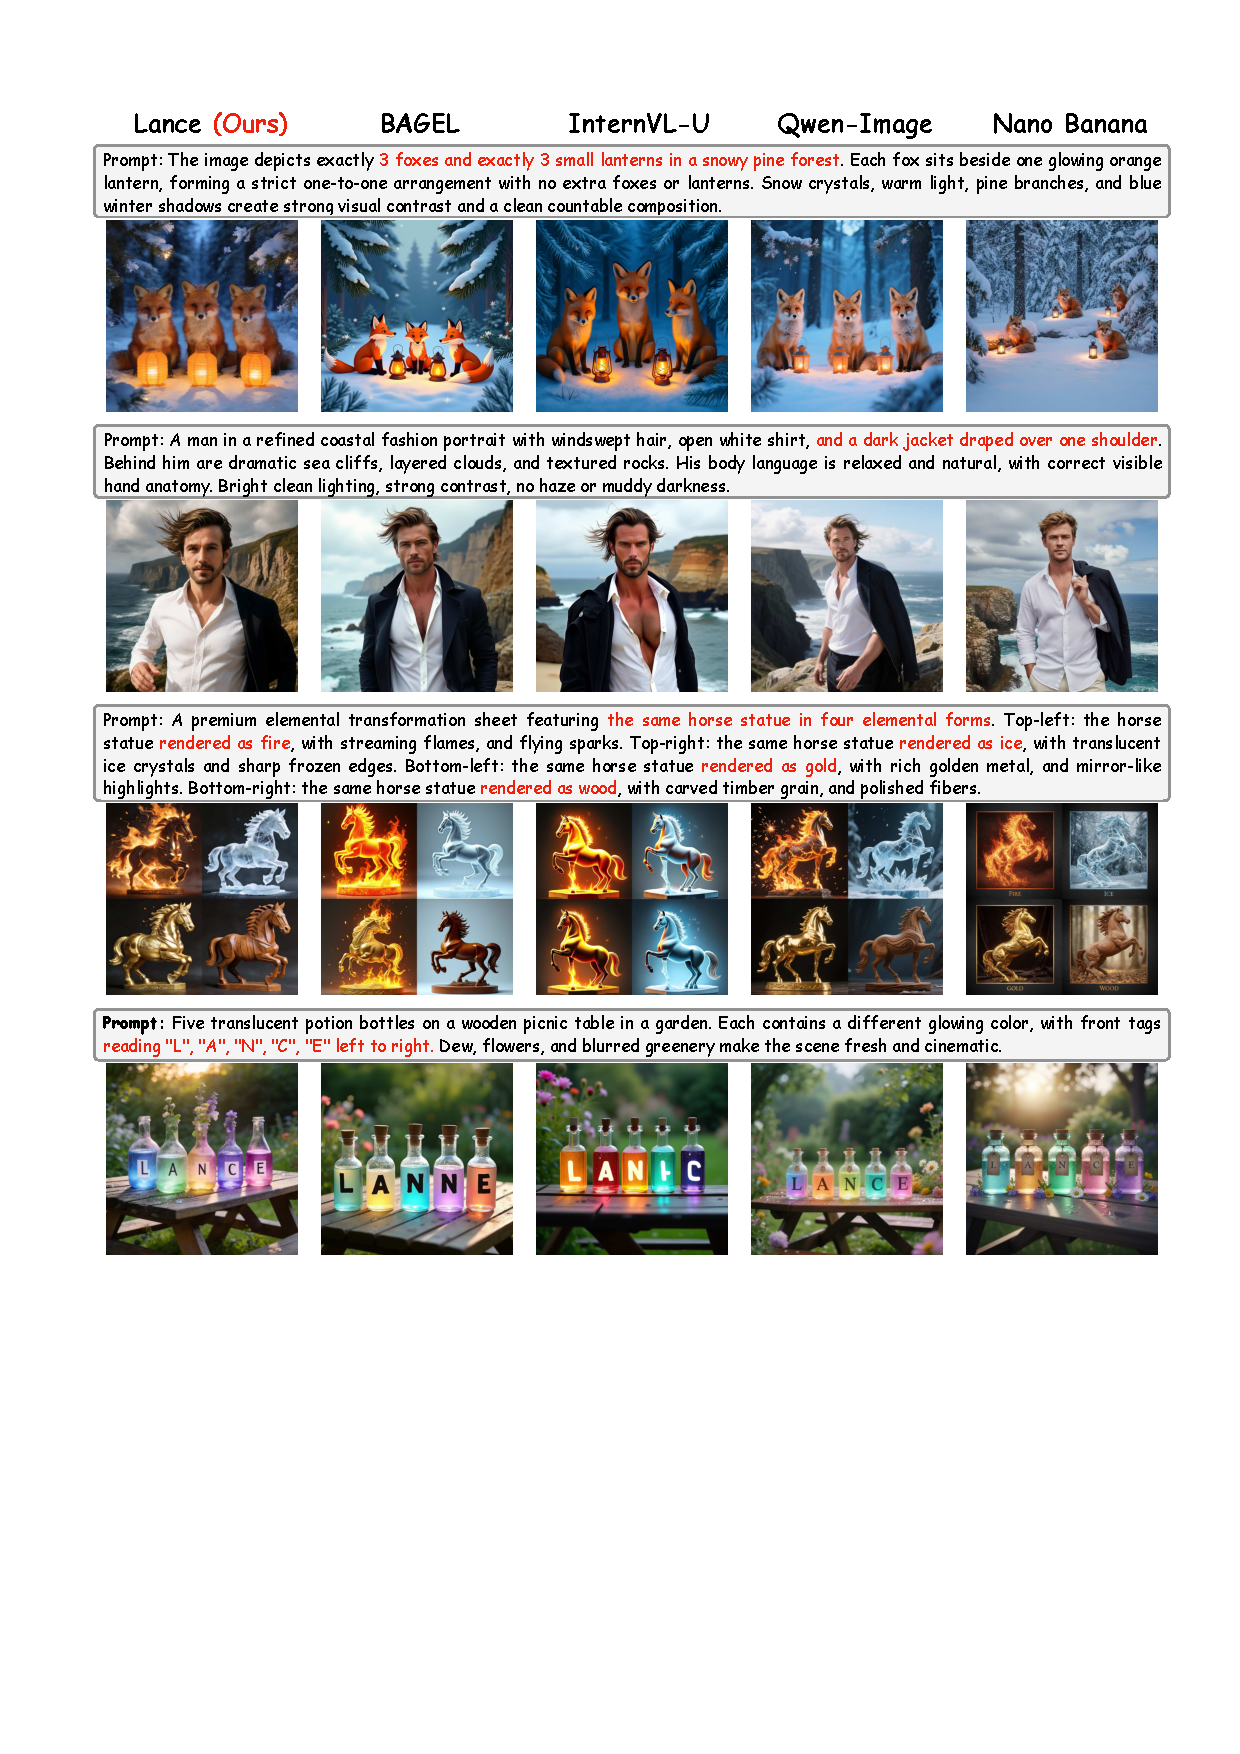
\includegraphics[width=1\textwidth]{figs/T2I-baseline.pdf} 
    \caption{\textbf{T2I qualitative comparison.} 
    %Lance demonstrates stronger image-text alignment than existing unified multimodal models (Bagel \cite{deng2025emerging}, InternVL-U \cite{tian2026internvlu}), and achieves comparable performance with $20$B Qwen-Image  ~\cite{wu2025qwen} and  commercial closed-source model Nano Banana \cite{Gemini3pro}.
    Instructions that are correctly reflected in our results but missed or incorrectly rendered by some baseline models are highlighted in {\color{red}{\textbf{red}}}.
    }
    \label{fig:T2I-baseline}
\end{figure*}







%\subsubsection{Experimental Settings}

Lance is implemented upon Qwen2.5-VL 3B \cite{Qwen2.5-VL}, using its weights to initialize the visual understanding encoder and the multimodal context backbones $\mathrm{LLM}_{\mathrm{UND}}$ and $\mathrm{LLM}_{\mathrm{GEN}}$. For the visual generation encoder, we adopt the 3D causal VAE encoder from Wan2.2 \cite{wan2025wan}, to support a unified processing of image and video modalities.
Following prior work \cite{ho2022classifier}, we also adopt classifier-free guidance (CFG) for visual and text conditions. During the PT stage, for text-to-image generation data, the text condition is dropped with a probability of $10\%$.
During the CT and SFT stages, for multimodal conditions, the full condition is dropped with a probability of $5\%$, while the text-only condition is additionally dropped with a probability of $5\%$ and the visual condition is retained.
During inference, the CFG scale for text conditions in generation tasks is set to $4$. Unless otherwise specified, the image input resolution is set to $768 \times 768$, while videos are sampled at $480p$ resolution with a frame rate of $12$ fps.



\subsection{Main Results}




\subsubsection{Image Generation}

\textbf{Quantitative Results.}
We evaluate the image generation capability of Lance on GenEval~\cite{ghosh2023geneval} and DPG-Bench~\cite{hu2024ella}. As shown in \Cref{tab:image_generation_combined}, Lance achieves top-tier performance among unified models on GenEval, matching the best overall score ($\textbf{0.90}$) while showing strong compositional ability on counting, colors, and spatial position. On DPG-Bench, Lance obtains competitive overall performance and performs particularly well on relation modeling, indicating its ability to preserve fine-grained semantic consistency under complex prompts. These results suggest that Lance can effectively support high-quality image synthesis within a unified multimodal framework, despite using only $3$B activated parameters.



\textbf{Qualitative Results.}
We conduct a qualitative comparison of Lance with $7$B Bagel \cite{deng2025emerging}, $1.7$B InternVL-U \cite{tian2026internvlu}, $20$B Qwen-Image  ~\cite{wu2025qwen} and Nano Banana \cite{Gemini3pro}. 
As shown in \Cref{fig:T2I-baseline}, compared with open-source unified multimodal baselines such as Bagel \cite{deng2025emerging} and InternVL-U \cite{tian2026internvlu}, Lance demonstrates stronger visual aesthetics and image-text alignment (\eg, lantern count in $1$-st case,
jacket draped over one shoulder in $2$-nd case).
Overall, Lance generates significantly higher-quality images than Bagel \cite{deng2025emerging} and InternVL-U \cite{tian2026internvlu}, and achieves comparable performance with the $20$B large-scale model Qwen-Image  ~\cite{wu2025qwen} and the commercial closed-source model Nano Banana \cite{Gemini3pro}.





\begin{table*}[!t]
\centering
\small
\setlength{\tabcolsep}{3.0pt}
\renewcommand{\arraystretch}{1.10}

% Local vertical separator. It appears only in normal/header rows,
% and disappears automatically in section-title rows with \multicolumn.
\newcommand{\vbenchsep}{\rule[-0.35em]{0.35pt}{1.55em}}

%========================
% Upper sub-table
%========================
\resizebox{0.9\textwidth}{!}{
\begin{tabular}{@{}l c c *{10}{c}@{}}
\toprule
\multicolumn{13}{c}{\textbf{(a) VBench Metrics Part I}} \\
\midrule
\multirow{1}{*}{\textbf{Models}}
& \multirow{1}{*}{\textbf{Params.}}
& \vbenchsep
& \makecell[c]{\textbf{Quality}\\\textbf{Score}}
& \makecell[c]{\textbf{Semantic}\\\textbf{Score}}
& \makecell[c]{\textbf{Subj.}\\\textbf{Consist.}}
& \makecell[c]{\textbf{Bkg.}\\\textbf{Consist.}}
& \makecell[c]{\textbf{Temp.}\\\textbf{Flicker.}}
& \makecell[c]{\textbf{Motion}\\\textbf{Smooth.}}
& \makecell[c]{\textbf{Dynamic}\\\textbf{Degree}}
& \makecell[c]{\textbf{Aesthetic}\\\textbf{Quality}}
& \makecell[c]{\textbf{Imaging}\\\textbf{Quality}}
& \makecell[c]{\textbf{Object}\\\textbf{Class}} \\
\midrule

\multicolumn{13}{@{}>{\columncolor{gray!12}}c@{}}{\textit{Generation-only Models}} \\

ModelScope \cite{wang2023modelscope}
& 1.7B
& \vbenchsep
& 78.05 & 66.54 & 89.87 & 95.29 & 98.28 & 95.79 & 66.39 & 52.06 & 58.57 & 82.25 \\

LaVie \cite{wang2025lavie}
& 3B
& \vbenchsep
& 78.78 & 70.31 & 91.41 & 97.47 & 98.30 & 96.38 & 49.72 & 54.94 & 61.90 & 91.82 \\

Show-1 \cite{zhang2025show}
& 6B
& \vbenchsep
& 80.42 & 72.98 & 95.53 & 98.02 & 99.12 & 98.24 & 44.44 & 57.35 & 58.66 & 93.07 \\

AnimateDiff-V2 \cite{guo2023animatediff}
& --
& \vbenchsep
& 82.90 & 69.75 & 95.30 & 97.68 & 98.75 & 97.76 & 40.83 & 67.16 & 70.10 & 90.90 \\

VideoCrafter-2.0 \cite{chen2024videocrafter2}
& --
& \vbenchsep
& 82.20 & 73.42 & 96.85 & 98.22 & 98.41 & 97.73 & 42.50 & 63.13 & 67.22 & 92.55 \\

CogVideoX \cite{yang2024cogvideox}
& 5B
& \vbenchsep
& 82.75 & 77.04 & 96.23 & 96.52 & 98.66 & 96.92 & 70.97 & 61.98 & 62.90 & 85.23 \\

Kling \cite{Kling2024}
& --
& \vbenchsep
& 83.39 & 75.68 & 98.33 & 97.60 & 99.30 & 99.40 & 46.94 & 61.21 & 65.62 & 87.24 \\

Open-Sora-2.0 \cite{opensora2}
& --
& \vbenchsep
& 82.10 & 80.14 & 98.75 & 98.00 & 99.40 & 99.49 & 20.74 & 64.33 & 65.62 & 94.50 \\

Gen-3 \cite{RunwayGen32024}
& --
& \vbenchsep
& 84.11 & 75.17 & 97.10 & 96.62 & 98.61 & 99.23 & 60.14 & 63.34 & 66.82 & 87.81 \\

Step-Video-T2V \cite{ma2025step}
& 30B
& \vbenchsep
& 84.46 & 71.28 & 98.05 & 97.67 & 99.40 & 99.08 & 53.06 & 61.23 & 70.63 & 80.56 \\

HunyuanVideo \cite{wu2025hunyuanvideo}
& --
& \vbenchsep
& 85.07 & 76.88 & 97.22 & 97.60 & 99.39 & 99.05 & 71.94 & 60.28 & 67.24 & 83.48 \\

Wan2.1-T2V \cite{wan2025wan}
& 14B
& \vbenchsep
& 85.59 & 76.11 & 97.52 & 98.09 & 99.46 & 98.30 & 65.46 & 66.07 & 69.43 & 86.28 \\

\midrule
\multicolumn{13}{@{}>{\columncolor{gray!12}}c@{}}{\textit{Unified Models}} \\

HaploOmni \cite{xiao2025haploomni}
& 7B
& \vbenchsep
& -- & -- & \underline{96.40} & \underline{97.60} & -- & 96.80 & 65.30 & -- & -- & -- \\

Emu3 \cite{wang2024emu3}
& 8B
& \vbenchsep
& -- & -- & 95.32 & \textbf{97.69} & -- & \textbf{98.93} & \textbf{79.27} & 59.64 & -- & 86.17 \\

VILA-U \cite{wu2024vila}
& 7B
& \vbenchsep
& 76.26 & 65.04 & -- & -- & -- & -- & -- & -- & -- & -- \\

Show-o2 \cite{xie2025show}
& 2B
& \vbenchsep
& 82.10 & 78.31 & \textbf{97.28} & 96.78 & 97.68
& 98.25 & 40.83 & \underline{65.15} & \textbf{67.06} & 94.81 \\

TUNA \cite{liu2025tuna}
& 1.5B
& \vbenchsep
& \underline{84.32} & \underline{83.04} & 95.99 & 96.72 & \underline{98.02}
& \underline{98.33} & 69.39 & \textbf{65.88} & \underline{66.83} & \underline{95.41} \\

\rowcolor{rowblue}
\textbf{Lance (Ours)}
& \textbf{3B}
& \vbenchsep
& \textbf{85.14} & \textbf{84.96} & 94.52 & 94.28 & \textbf{99.66}
& 95.93 & \underline{75.83} & 64.33 & 66.78 & \textbf{96.58} \\

\bottomrule
\end{tabular}}

\vspace{0.6em}

%========================
% Lower sub-table
%========================
\resizebox{0.9\textwidth}{!}{
\begin{tabular}{@{}l c c *{9}{c}@{}}
\toprule
\multicolumn{12}{c}{\textbf{(b) VBench Metrics Part II}} \\
\midrule
\multirow{1}{*}{\textbf{Models}}
& \multirow{1}{*}{\textbf{Params.}}
& \vbenchsep
& \makecell[c]{\textbf{Multi.}\\\textbf{Objects}}
& \makecell[c]{\textbf{Human}\\\textbf{Action}}
& \makecell[c]{\textbf{Color}}
& \makecell[c]{\textbf{Spatial}\\\textbf{Relation}}
& \makecell[c]{\textbf{Scene}}
& \makecell[c]{\textbf{Appear.}\\\textbf{Style}}
& \makecell[c]{\textbf{Temp.}\\\textbf{Style}}
& \makecell[c]{\textbf{Overall}\\\textbf{Consist.}}
& \makecell[c]{\textbf{Total}\\\textbf{Score}$\uparrow$} \\
\midrule

\multicolumn{12}{@{}>{\columncolor{gray!12}}c@{}}{\textit{Generation-only Models}} \\

ModelScope \cite{wang2023modelscope}
& 1.7B
& \vbenchsep
& 38.98 & 92.40 & 81.72 & 33.68 & 39.26 & 23.39 & 25.37 & 25.67 & 75.75 \\

LaVie \cite{wang2025lavie}
& 3B
& \vbenchsep
& 33.32 & 96.80 & 86.39 & 34.09 & 52.69 & 23.56 & 25.93 & 26.41 & 77.08 \\

Show-1 \cite{zhang2025show}
& 6B
& \vbenchsep
& 45.47 & 95.60 & 86.35 & 53.50 & 47.03 & 23.06 & 25.28 & 27.46 & 78.93 \\

AnimateDiff-V2 \cite{guo2023animatediff}
& --
& \vbenchsep
& 36.88 & 92.60 & 87.47 & 34.60 & 50.19 & 22.42 & 26.03 & 27.04 & 80.27 \\

VideoCrafter-2.0 \cite{chen2024videocrafter2}
& --
& \vbenchsep
& 40.66 & 95.00 & 92.92 & 35.86 & 55.29 & 25.13 & 25.84 & 28.23 & 80.44 \\

CogVideoX \cite{yang2024cogvideox}
& 5B
& \vbenchsep
& 62.11 & 99.40 & 82.81 & 66.35 & 53.20 & 24.91 & 25.38 & 27.59 & 81.61 \\

Kling \cite{Kling2024}
& --
& \vbenchsep
& 68.05 & 93.40 & 89.90 & 73.03 & 50.86 & 19.62 & 24.17 & 26.42 & 81.85 \\

Open-Sora-2.0 \cite{opensora2}
& --
& \vbenchsep
& 77.72 & 95.40 & 85.98 & 76.18 & 52.71 & 22.98 & 25.91 & 27.57 & 81.71 \\

Gen-3 \cite{RunwayGen32024}
& --
& \vbenchsep
& 53.64 & 96.40 & 80.90 & 65.09 & 54.57 & 24.31 & 24.71 & 26.69 & 82.32 \\

Step-Video-T2V \cite{ma2025step}
& 30B
& \vbenchsep
& 50.55 & 94.00 & 88.25 & 71.47 & 24.38 & 23.17 & 26.01 & 27.12 & 81.83 \\

HunyuanVideo \cite{wu2025hunyuanvideo}
& --
& \vbenchsep
& 66.71 & 94.40 & 89.79 & 72.13 & 54.46 & 22.21 & 24.52 & 26.95 & 83.43 \\

Wan2.1-T2V \cite{wan2025wan}
& 14B
& \vbenchsep
& 69.58 & 95.40 & 88.59 & 75.39 & 45.75 & 22.64 & 23.19 & 25.91 & 83.69 \\

\midrule
\multicolumn{12}{@{}>{\columncolor{gray!12}}c@{}}{\textit{Unified Models}} \\

HaploOmni \cite{xiao2025haploomni}
& 7B
& \vbenchsep
& -- & -- & -- & -- & 34.60 & -- & -- & -- & 78.10 \\

Emu3 \cite{wang2024emu3}
& 8B
& \vbenchsep
& 44.64 & 77.71 & -- & 68.73 & 37.11 & 20.92 & -- & -- & 80.96 \\

VILA-U \cite{wu2024vila}
& 7B
& \vbenchsep
& -- & -- & -- & -- & -- & -- & -- & -- & 74.01 \\

Show-o2 \cite{xie2025show}
& 2B
& \vbenchsep
& 76.01 & 95.20 & 80.89 & 62.61 & 57.67 & \textbf{23.29} & \underline{25.27} & 27.00 & 81.34 \\

TUNA \cite{liu2025tuna}
& 1.5B
& \vbenchsep
& \underline{92.31} & \underline{97.50} & \underline{87.67} & \underline{78.12} & \underline{58.59}
& \underline{23.18} & 24.68 & \textbf{27.71} & \underline{84.06} \\

\rowcolor{rowblue}
\textbf{Lance (Ours)}$^\dagger$
& \textbf{3B}
& \vbenchsep
& \textbf{93.86} & \textbf{97.80} & \textbf{92.61} & \textbf{93.61} & \textbf{64.75}
& 23.14 & \textbf{25.53} & \underline{27.04} & \textbf{85.11} \\
\bottomrule
\end{tabular}}
\caption{\textbf{Video generation results on VBench.}
$^\dagger$ refers to methods using LLM rewriters.
\textbf{Bold}: best results among unified models.
\underline{Underline}: second-best among unified models.}
\label{tab:vbench_full}
\end{table*}

\begin{figure*}[!t]
    \centering
    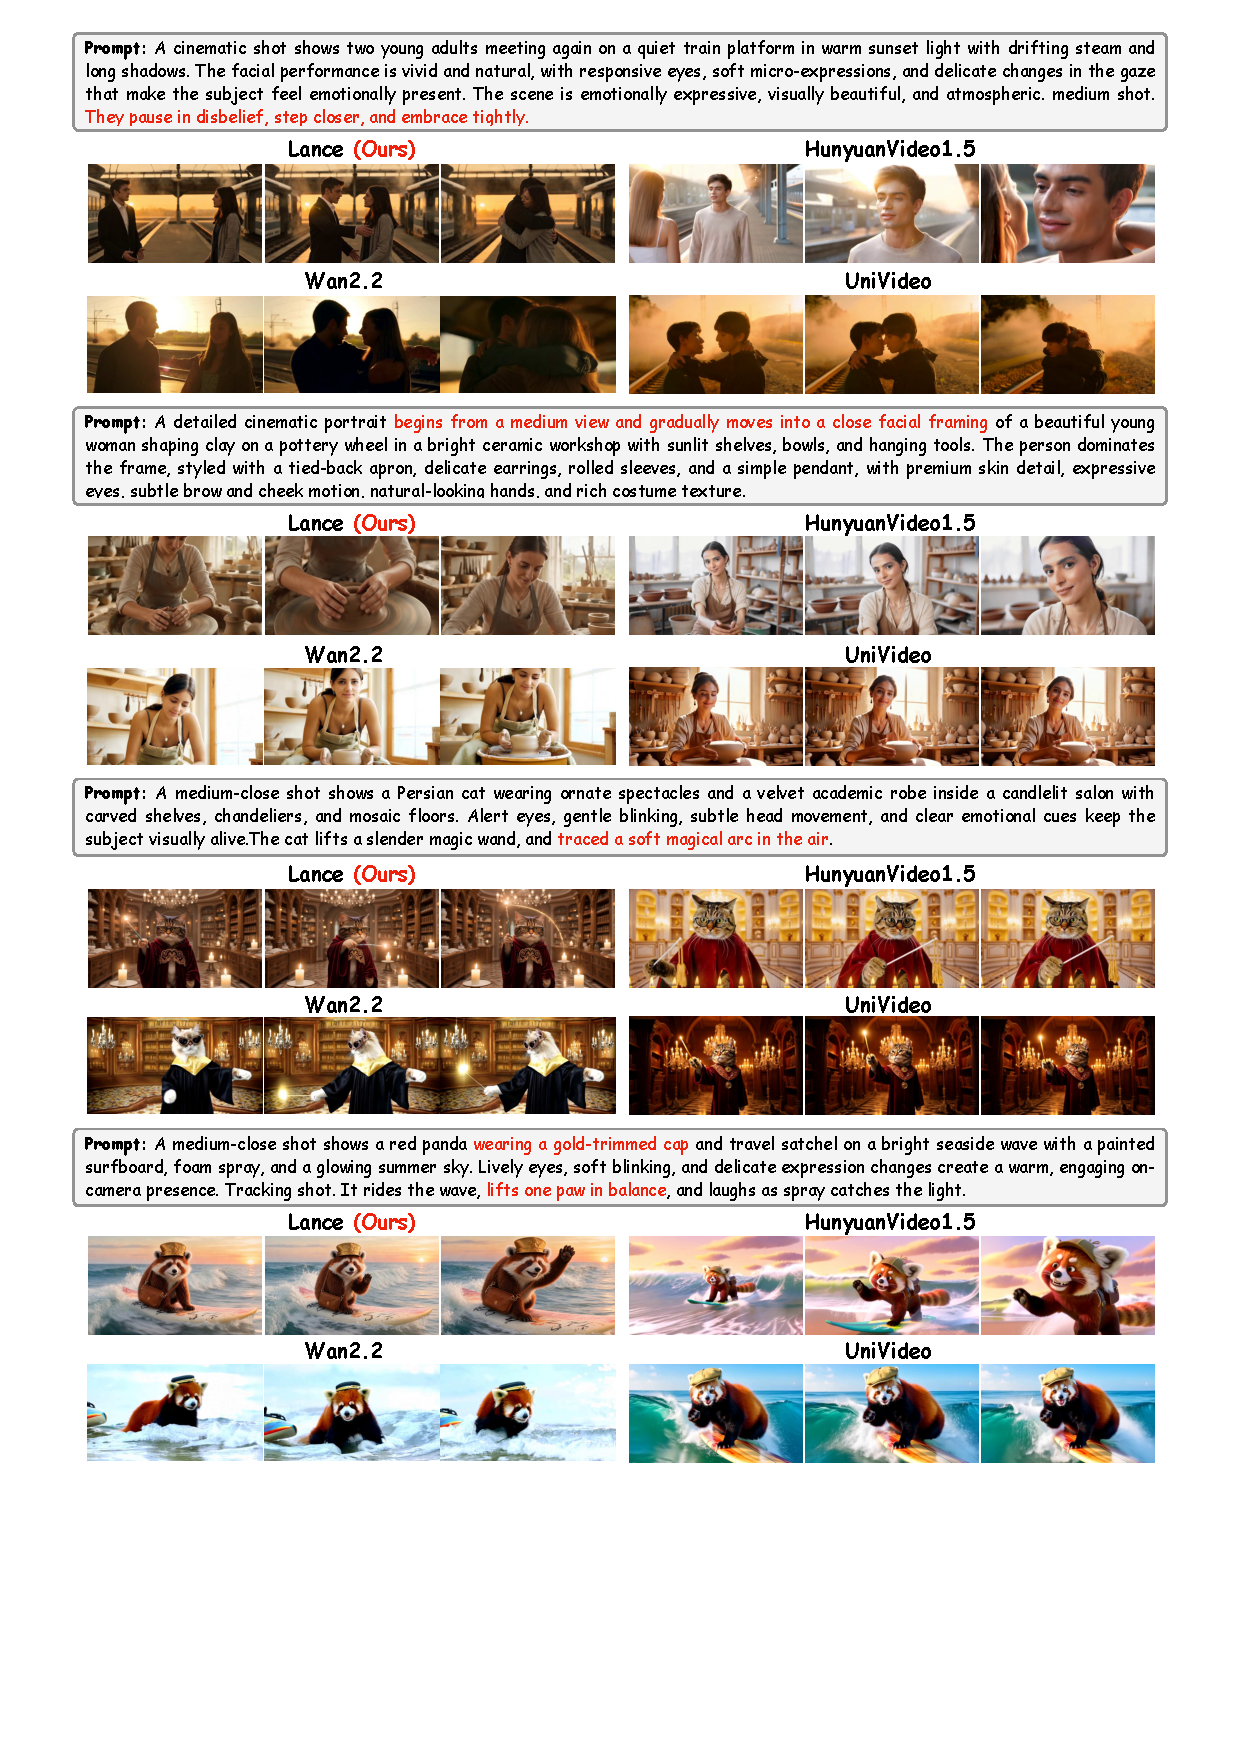
\includegraphics[width=0.96\textwidth]{figs/T2V-baseline.pdf}
    \caption{\textbf{T2V qualitative comparison.}
    Instructions that are correctly reflected in our results but missed or incorrectly rendered by some baseline models are highlighted in {\color{red}{\textbf{red}}}.
    }
    %Lance exhibits stronger visual aesthetics and more precise camera transitions.}
    \label{fig:T2V-baseline}
\end{figure*}


\subsubsection{Video Generation}


\textbf{Quantitative Results.}
We evaluate the text-to-video generation capability of Lance on VBench~\cite{huang2024vbench}. As shown in \Cref{tab:vbench_full}, Lance achieves the best Total Score ($\textbf{85.11}$) among unified models with only $3$B activated parameters. Beyond the overall score, Lance also shows strong performance across both quality-oriented and semantic-oriented dimensions, including visual quality, object grounding, color consistency, spatial relationships, scene understanding, and temporal style. These results indicate that the proposed unified framework effectively supports compositional video generation and text-video alignment, while scaling naturally from image generation to more challenging spatiotemporal generation tasks.


\textbf{Qualitative Results.}
We conduct a qualitative comparison between Lance and $8.3$B HunyuanVideo1.5 \cite{wu2025hunyuanvideo}, $5$B Wan2.2-TI2V \cite{wan2025wan}, and $7$B UniVideo \cite{wei2025univideo}.
As shown in \Cref{fig:T2V-baseline}, the generated videos exhibit strong semantic fidelity, coherent motion, and appealing visual quality. In challenging cases involving complex human interactions (\eg, $1$-st case, ``two adults hugging"), or explicit camera transitions (\eg, $2$-nd case, from a ``medium view" to ``close facial framing"), our model follows the prompt accurately and produces videos with stable visual texture and consistent temporal evolution. These examples further demonstrate the effectiveness of the unified architecture for high-quality text-to-video generation.




\begin{table*}[!t]
\centering
\small
\setlength{\tabcolsep}{3.0pt}
\renewcommand{\arraystretch}{1.10}

% Local vertical separator. It appears only in normal/header rows,
% and disappears automatically in section-title rows with \multicolumn.
\newcommand{\geditsep}{\rule[-0.35em]{0.35pt}{1.55em}}

\resizebox{\textwidth}{!}{
\begin{tabular}{@{}l c c *{12}{c}@{}}
\toprule

\multirow{2}{*}{\textbf{Models}}
& \multirow{2}{*}{\textbf{Params.}}
& \geditsep
& \multicolumn{12}{c}{\textbf{GEdit-Bench}} \\
\cmidrule(lr){4-15}
&
& \geditsep
& \textbf{BC} & \textbf{CA} & \textbf{MM} & \textbf{MC} & \textbf{PB} & \textbf{ST}
& \textbf{SA} & \textbf{SR} & \textbf{SRp} & \textbf{TM} & \textbf{TT} & \textbf{Avg/G\_O} \\
\midrule

\multicolumn{15}{@{}>{\columncolor{gray!12}}c@{}}{\textit{Generation-only Models}} \\

Gemini 2.0 \cite{team2024gemini}
& --
& \geditsep
& -- & -- & -- & -- & -- & -- & -- & -- & -- & -- & -- & 6.32 \\

GPT Image 1 \cite{openai2025gptimage1}
& --
& \geditsep
& 6.96 & 6.85 & 7.10 & 5.41 & 6.74 & 7.44 & 7.51 & 8.73 & 8.55 & 8.45 & 8.69 & 7.49 \\

Qwen-Image-Edit \cite{wu2025qwen}
& 20B
& \geditsep
& 8.23 & 8.30 & 7.33 & 8.05 & 7.49 & 6.74 & 8.57 & 8.09 & 8.29 & 8.48 & 8.50 & 8.01 \\

\midrule
\multicolumn{15}{@{}>{\columncolor{gray!12}}c@{}}{\textit{Unified Models}} \\

Lumina-DiMOO \cite{xin2025lumina}
& 8B
& \geditsep
& 3.43 & 4.27 & 3.08 & 2.77 & 4.74 & 5.19 & 4.44 & 3.80 & 4.38 & 2.68 & 4.20 & 3.91 \\

Ovis-U1 \cite{wang2025ovis}
& 1.2B
& \geditsep
& \underline{7.49} & 6.88 & 6.21 & 4.79 & 5.98 & \underline{6.46}
& 7.49 & \underline{7.25} & \underline{7.27} & 4.48 & 6.31 & 6.42 \\

BAGEL \cite{deng2025emerging}
& 7B
& \geditsep
& 7.32 & 6.91 & 6.38 & 4.75 & 4.57 & 6.15
& \textbf{7.90} & 7.16 & 7.02 & \underline{7.32} & 6.22 & 6.52 \\

InternVL-U \cite{tian2026internvlu}
& 1.7B
& \geditsep
& 7.08 & 7.05 & 6.38 & \underline{7.02} & \underline{6.03} & 6.27
& 7.13 & 6.55 & 6.33 & 6.59 & \underline{6.85} & 6.66 \\

InternVL-U (w/ CoT) \cite{tian2026internvlu}
& 1.7B
& \geditsep
& 7.05 & \textbf{7.87} & \underline{6.50} & 6.99 & 5.77 & 6.10
& 7.33 & 7.16 & 7.12 & \textbf{7.36} & 6.46 & \underline{6.88} \\

\rowcolor{rowblue}
\textbf{Lance (Ours)}
& \textbf{3B}
& \geditsep
& \textbf{7.73} & \underline{7.74} & \textbf{7.28} & \textbf{7.83} & \textbf{7.50} & \textbf{7.03}
& \underline{7.64} & \textbf{7.85} & \textbf{7.71} & 4.46 & \textbf{7.57} & \textbf{7.30} \\

\bottomrule
\end{tabular}
}
\caption{\textbf{
Image editing results on GEdit-Bench.}
% BC=Background Change, CA=Color Alteration, MM=Material Modification, MC=Motion Change,
% PB=Portrait Beautification, ST=Style Transfer, SA=Subject Addition, SR=Subject Removal,
% SRp=Subject Replacement, TM=Text Modification, and TT=Tone Transfer.
\textbf{Bold}: best results among unified models.
\underline{Underline}: second-best among unified models.}
\label{tab:gedit_bench}
\end{table*}

\begin{figure}[!t]
    \centering
    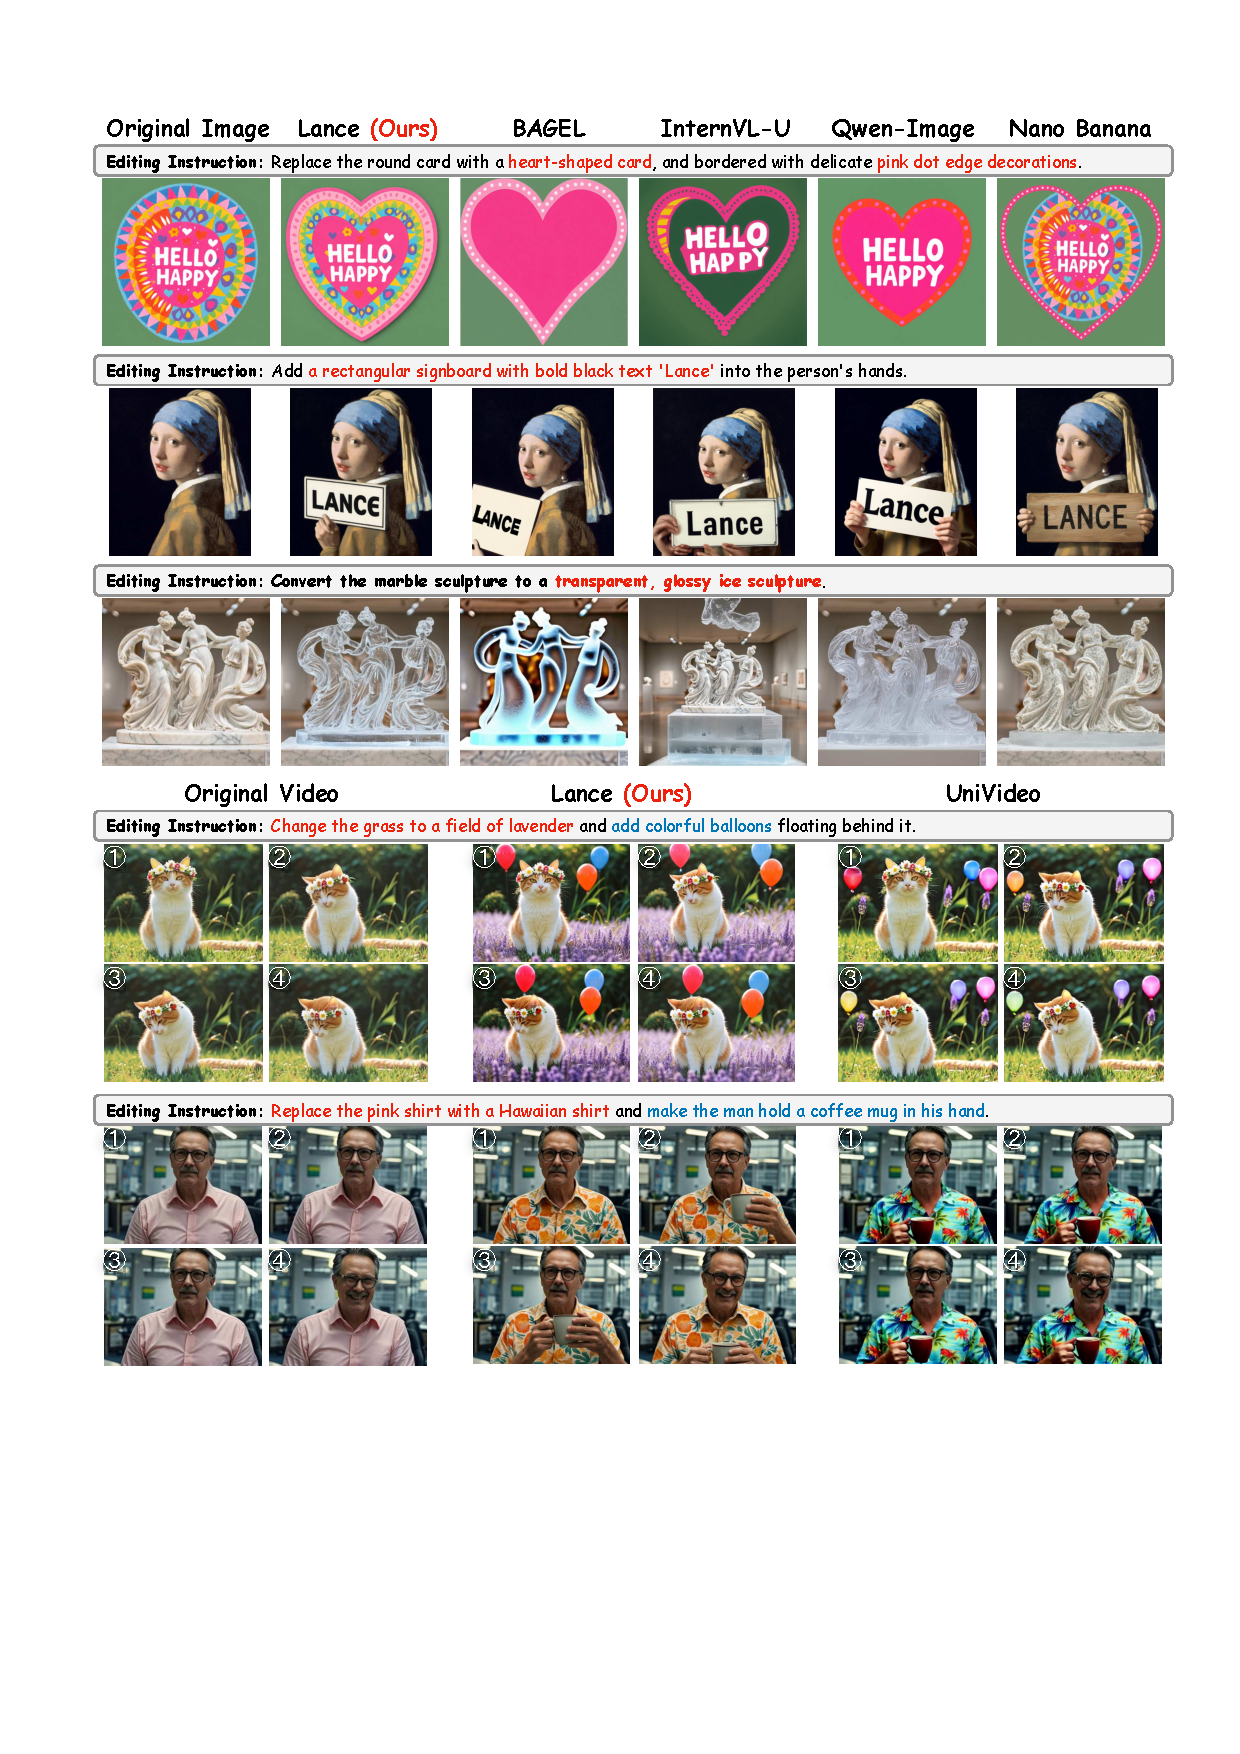
\includegraphics[width=\linewidth]{figs/edit-baseline.pdf}
    \caption{\textbf{Multimodal editing qualitative comparison.}    
    Lance performs precise image editing with realistic texture and structure preservation, and supports temporally coherent video editing with natural motion dynamics.}
    \label{fig:multimodal_editing_qual}
\end{figure}


\subsubsection{Multimodal Editing}

\textbf{Quantitative Results.}
We evaluate the image editing capability of our model on GEdit-Bench \cite{liu2025step1x}. As shown in \Cref{tab:gedit_bench}, our model achieves the best Avg/G$\_$O score (7.30) among unified models, demonstrating strong overall editing performance under a compact parameter budget. In particular, our model obtains the best results in several key editing categories, including background change, material modification, motion change, portrait beautification, subject removal, replacement, and tone transfer.  These results suggest that the proposed unified framework can effectively support a broad range of image editing operations. We also observe that Lance is relatively weaker on text modification, indicating that text-specific editing remains an important direction for future improvement.



\textbf{Qualitative Results.}
We further provide qualitative results for both image and video editing in \Cref{fig:multimodal_editing_qual}.
For image editing, Lance achieves visually coherent image editing with well-preserved structures and realistic textures, \eg, the plausible hand geometry and fine details in the $2$-nd case. For video editing, Lance performs accurate multi-attribute modifications while maintaining natural motion dynamics, such as the temporally consistent hand movement of the person holding a cup in the last case. Overall, these results demonstrate Lance's high-fidelity editing ability in both spatial realism and temporal coherence, highlighting the potential of unified models for multimodal editing.



\begin{table*}[!t]
\centering
\small
\setlength{\tabcolsep}{2.4pt}
\renewcommand{\arraystretch}{1.10}

% Local vertical separator. It appears only in normal/header rows,
% and disappears automatically in section-title rows with \multicolumn.
\providecommand{\mvbenchsep}{\rule[-0.35em]{0.35pt}{1.55em}}

\resizebox{\textwidth}{!}{
\begin{tabular}{@{}l c c *{20}{c}@{}}
\toprule

\multirow{2}{*}{\textbf{Models}}
& \multirow{2}{*}{\textbf{Params.}}
& \mvbenchsep
& \multicolumn{20}{c}{\textbf{MVBench}} \\
\cmidrule(lr){4-23}
&
& \mvbenchsep
& \textbf{AS} & \textbf{AP} & \textbf{AA} & \textbf{FA} & \textbf{UA}
& \textbf{OE} & \textbf{OI} & \textbf{OS} & \textbf{MD} & \textbf{AL}
& \textbf{ST} & \textbf{AC} & \textbf{MC} & \textbf{MA} & \textbf{SC}
& \textbf{CO} & \textbf{EN} & \textbf{ER} & \textbf{CI} & \textbf{Avg.$\uparrow$} \\
\midrule

\multicolumn{23}{@{}>{\columncolor{gray!12}}c@{}}{\textit{Understanding-only Models}} \\

Video-LLaMA \cite{zhang-etal-2023-video}
& 7B
& \mvbenchsep
& 27.5 & 25.5 & 51.0 & 29.0 & 39.0
& 48.0 & 40.5 & 38.0 & 22.5 & 22.5
& 43.0 & 34.0 & 22.5 & 32.5 & 45.5
& 40.0 & 30.0 & 21.0 & 37.0 & 34.1 \\

LLaMA-Adapter \cite{zhang2023llamaadapter}
& 7B
& \mvbenchsep
& 23.0 & 28.0 & 51.0 & 30.0 & 33.0
& 53.5 & 32.5 & 33.5 & 25.5 & 21.5
& 30.5 & 29.0 & 22.5 & 41.5 & 39.5
& 31.5 & 22.5 & 28.0 & 32.0 & 31.7 \\

Video-ChatGPT \cite{Maaz2023VideoChatGPT}
& 7B
& \mvbenchsep
& 23.5 & 26.0 & 62.0 & 22.5 & 26.5
& 54.0 & 28.0 & 40.0 & 23.0 & 20.0
& 31.0 & 30.5 & 25.5 & 39.5 & 48.5
& 33.0 & 29.5 & 26.0 & 35.5 & 32.7 \\

VideoChat \cite{li2025videochat}
& 7B
& \mvbenchsep
& 33.5 & 26.5 & 56.0 & 33.5 & 40.5
& 53.0 & 40.5 & 30.0 & 25.5 & 27.0
& 48.5 & 35.0 & 20.5 & 42.5 & 46.0
& 41.0 & 23.5 & 23.5 & 36.0 & 35.5 \\

VideoChat2 \cite{li2024mvbench}
& 7B
& \mvbenchsep
& 66.0 & 47.5 & 83.5 & 49.5 & 60.0
& 58.0 & 71.5 & 42.5 & 23.0 & 23.0
& 88.5 & 39.0 & 42.0 & 58.5 & 44.0
& 36.5 & 35.0 & 40.5 & 65.5 & 51.1 \\

ST-LLM \cite{liu2024st}
& 7B
& \mvbenchsep
& 66.0 & 53.5 & 84.0 & 44.0 & 58.5
& 80.5 & 73.5 & 38.5 & 42.5 & 31.0
& 86.5 & 36.5 & 56.5 & 78.5 & 43.0
& 46.5 & 34.5 & 41.5 & 58.5 & 54.9 \\

GPT-4V \cite{openai2023gpt4v}
& --
& \mvbenchsep
& 55.5 & 63.5 & 72.0 & 46.5 & 73.5
& 18.5 & 59.0 & 29.5 & 12.0 & 40.5
& 83.5 & 39.0 & 12.0 & 22.5 & 45.0
& 52.0 & 31.0 & 59.0 & 11.0 & 43.5 \\

PLLaVA \cite{xu2024pllava}
& 34B
& \mvbenchsep
& 67.5 & 53.0 & 82.0 & 47.0 & 79.0
& 68.5 & 67.5 & 36.5 & 37.5 & 49.5
& 91.0 & 40.5 & 43.0 & 70.0 & 51.5
& 66.5 & 39.5 & 63.5 & 59.0 & 58.1 \\

Video-CCAM \cite{fei2024video}
& 9B
& \mvbenchsep
& 83.0 & 67.0 & 89.5 & 49.0 & 72.0
& 86.5 & 81.0 & 45.0 & 28.0 & 29.0
& 90.0 & 59.0 & 67.0 & 85.0 & 63.5
& 77.0 & 34.0 & 73.5 & 59.0 & 64.6 \\

Qwen2.5-VL \cite{Qwen2.5-VL}
& 3B
& \mvbenchsep
& -- & -- & -- & -- & --
& -- & -- & -- & -- & --
& -- & -- & -- & -- & --
& -- & -- & -- & -- & 67.0 \\

TimeMarker \cite{chen2024timemarker}
& 8B
& \mvbenchsep
& 79.0 & 74.5 & 89.0 & 53.5 & 77.0
& 94.0 & 76.0 & 41.5 & 52.5 & 47.0
& 91.5 & 53.0 & 76.5 & 92.5 & 57.0
& 70.5 & 23.5 & 53.5 & 82.5 & 67.4 \\

InternVideo2 \cite{wang2024internvideo2}
& 7B
& \mvbenchsep
& 86.0 & 70.0 & 87.0 & 56.0 & 75.0
& 91.0 & 86.0 & 40.0 & 48.0 & 53.0
& 90.0 & 41.0 & 73.0 & 92.0 & 52.0
& 56.0 & 33.0 & 57.0 & 74.0 & 67.3 \\

\midrule
\multicolumn{23}{@{}>{\columncolor{gray!12}}c@{}}{\textit{Unified Models}} \\

Show-o2 \cite{xie2025show}
& 1.5B
& \mvbenchsep
& \underline{63.8} & 59.5 & 63.5 & 40.0 & \underline{70.5}
& 54.5 & 66.0 & 36.5 & \underline{36.0} & 27.0
& \underline{88.0} & \underline{43.5} & 43.0 & 58.0 & \underline{44.5}
& \underline{54.0} & 28.5 & 39.5 & \underline{45.0} & 50.6 \\

Show-o2 \cite{xie2025show}
& 7B
& \mvbenchsep
& 60.1 & \underline{67.0} & 68.0 & 45.5 & \textbf{78.0}
& 51.0 & \textbf{73.5} & \textbf{44.5} & \underline{36.0} & \textbf{39.0}
& \textbf{92.5} & \textbf{51.5} & 36.0 & 59.5 & \textbf{52.0}
& \textbf{64.0} & \textbf{38.0} & \textbf{60.0} & 43.0 & \underline{55.7} \\

TUNA \cite{liu2025tuna}
& 1.5B
& \mvbenchsep
& -- & -- & -- & -- & --
& -- & -- & -- & -- & --
& -- & -- & -- & -- & --
& -- & -- & -- & -- & 54.4 \\

UniVideo \cite{wei2025univideo}
& 7B
& \mvbenchsep
& 54.3 & 41.5 & \textbf{77.5} & \textbf{50.0} & 62.5
& \underline{68.2} & 50.5 & \underline{37.5} & \underline{36.0} & 29.5
& 35.5 & 28.5 & \underline{52.5} & \underline{70.5} & 33.5
& 40.5 & \underline{37.5} & 36.5 & 38.0 & 46.3 \\

\rowcolor{rowblue}
\textbf{Lance (Ours)}
& \textbf{3B}
& \mvbenchsep
& \textbf{73.9} & \textbf{76.5} & \underline{71.5} & \underline{49.0} & 63.5
& \textbf{96.0} & \underline{72.5} & 33.0 & \textbf{63.5} & \underline{33.0}
& 86.0 & 41.0 & \textbf{82.0} & \textbf{97.5} & 43.0
& 47.5 & 31.5 & \underline{40.0} & \textbf{77.0} & \textbf{62.0} \\

\bottomrule
\end{tabular}
}
\caption{\textbf{Video understanding results on MVBench.}
\textbf{Bold}: best results among unified models.
\underline{Underline}: second-best among unified models.}
\label{tab:mvbench_main}
\end{table*}

\subsubsection{Multimodal Understanding}

\textbf{Quantitative Results.}
We evaluate the video understanding ability of Lance on MVBench \cite{li2024mvbench}, a widely used multi-choice benchmark for assessing temporal perception and video-centric understanding. 
As reported in \Cref{tab:mvbench_main}, Lance achieves the highest overall score (\textbf{62.0}) among existing unified multimodal models, with an approximately \textbf{11.3\%} relative improvement compared to the second-best unified model, Show-o2 7B \cite{xie2025show}. Lance also surpasses most of the specialized understanding models, with only half or even fewer parameters, indicating that unified multi-task training can preserve strong video understanding while enabling generation and editing capabilities.

\textbf{Qualitative Results.}
We present qualitative examples for image and video understanding in \Cref{fig:X2I,fig:X2V}.
Lance handles diverse understanding tasks, including OCR, knowledge-grounded reasoning, multi-image motion analysis, detailed video captioning, and action counting. The examples show that Lance can recognize fine-grained visual details, reason over static images, and capture temporal dynamics in videos. These results indicate that Lance maintains strong multimodal understanding ability while jointly supporting generation and editing within a unified model.


